\begin{figure}[H]
    \centering
    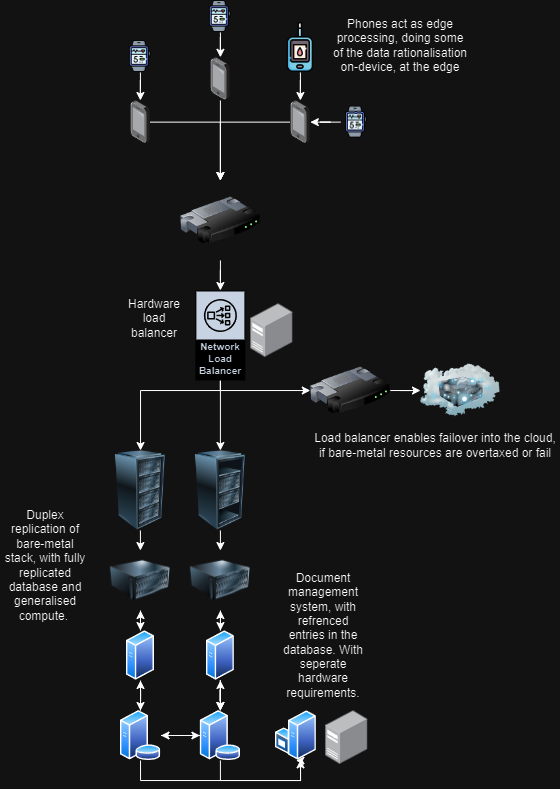
\includegraphics[width=0.6\textwidth]{as3_diagram.drawio.png}
    \caption{System Diagram}
\end{figure}

\section{Smartphones as Edge Computing Nodes}
Smartphones are utilized as edge compute nodes due to their advanced processing
capability and sensors.They preprocess information gathered from wearables by
performing information filtering, initial analysis, and significance
assessment. This not only enhances the quality of information sent to the
central server but also reduces the bandwidth needed for information
transmission. \cite{ning2020mobile}

\section{Processing Server and Database}
The central processing server performs detailed data analysis and complex
processing tasks. It is distinct yet closely integrated with the database to
facilitate seamless information flow between processing and storage components.
The server handles tasks such as:

\begin{itemize}
    \item Further analysis of preprocessed information from smartphones
    \item Application of machine learning algorithms
    \item Generation of actionable insights and reports
\end{itemize}

\noindent{}The database is seperatly hosted. This separation ensures dedicated resources
are available for process and storage functions, this seperation allows for more
specialised hardware to be used for the database, which can be optimised for
read and write operations. \cite{liu2024integrating}

\section{Load Balancer for Data Ingress}
A load balancer is employed to handle data incoming from multiple smartphone
edge nodes efficiently. This setup ensures that incoming information is spread
equally across available server resources, preventing server overload.

\section{Document Management System Integration}
The Document Management System is integrated with the database to facilitate
structured storage, retrieval, and management of documents. This integration
allows the system to manage large volumes of documents efficiently, providing
fast data retrieval and compliance with document retention policies and
regulations.

\section{Security and Compliance Measures}
Comprehensive security measures are integral to the architecture, including:

\begin{itemize}
    \item End-to-end encryption of information in transit and at rest
    \item Secure authentication mechanisms
    \item Rigorous access control
\end{itemize}

\noindent{}Compliance with data security laws such as GDPR is meticulously maintained to
ensure the system respects and protects user privacy throughout all operations.

\section{Scalability and Maintenance}
The architecture is designed to be scalable to accommodate an increased amount of
users and high data volumes. Regular updates and maintenance are planned to
enhance system functionality, address security vulnerabilities, and assure
sustained performance and reliability.